% `\addlegendentry{}` and `\addlegendentry{ }` keep their image with an empty
% text cell (height 0, depth = text depth); papers use it to pair two images
% per row with legend columns=2 (behaviour Z8).
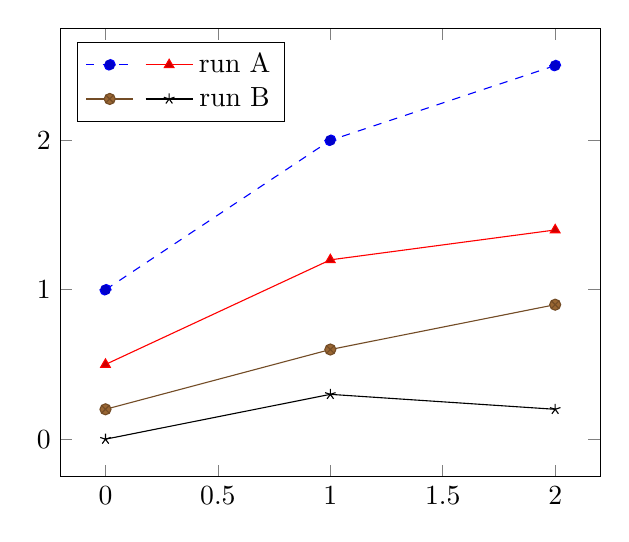
\begin{tikzpicture}
\begin{axis}[legend columns=2, legend pos=north west]
\addplot+[dashed] coordinates {(0,1) (1,2) (2,2.5)};
\addlegendentry{ }
\addplot+[mark=triangle*] coordinates {(0,0.5) (1,1.2) (2,1.4)};
\addlegendentry{run A}
\addplot+[] coordinates {(0,0.2) (1,0.6) (2,0.9)};
\addlegendentry{}
\addplot+[] coordinates {(0,0) (1,0.3) (2,0.2)};
\addlegendentry{run B}
\end{axis}
\end{tikzpicture}
